\documentclass{beamer}

\usepackage{comment}
\usepackage{color}
\usepackage{listings}
\usepackage{verbatim}
\usepackage{multicol}
\usepackage{booktabs}
\definecolor{green}{RGB}{0,128,0}

\def\EQ#1\EN{\begin{equation*}#1\end{equation*}}
\def\BA#1\EA{\begin{align*}#1\end{align*}}
\def\BS#1\ES{\begin{split*}#1\end{split*}}
\newcommand{\bc}{\begin{center}}
\newcommand{\ec}{\end{center}}
\newcommand{\eq}{\ =\ }
\newcommand{\degc}{$^\circ$C}

\def\p{\partial}
\def\qbs{\boldsymbol{q}}
\def\Dbs{\boldsymbol{D}}
\def\A{\mathcal A}
\def\gC{\mathcal C}
\def\gD{\mathcal D}
\def\gL{\mathcal L}
\def\M{\mathcal M}
\def\P{\mathcal P}
\def\Q{\mathcal Q}
\def\gR{\mathcal R}
\def\gS{\mathcal S}
\def\X{\mathcal X}
\def\bnabla{\boldsymbol{\nabla}}
\def\bnu{\boldsymbol{\nu}}
\renewcommand{\a}{{\alpha}}
%\renewcommand{\a}{{}}
\newcommand{\s}{{\sigma}}
\newcommand{\bq}{\boldsymbol{q}}
\newcommand{\bz}{\boldsymbol{z}}
\def\bPsi{\boldsymbol{\Psi}}

\def\Li{\textit{L}}
\def\Fb{\textbf{f}}
\def\Jb{\textbf{J}}
\def\cb{\textbf{c}}

\def\Dt{\Delta t}
\def\tpdt{{t + \Delta t}}
\def\bpsi{\boldsymbol{\psi}}
\def\dbpsi{\delta \boldsymbol{\psi}}
\def\bc{\textbf{c}}
\def\bx{\textbf{x}}
\def\dbc{\delta \textbf{c}}
\def\dbx{\delta \textbf{x}}
\def\arrows{\rightleftharpoons}

\newcommand{\bGamma}{\boldsymbol{\Gamma}}
\newcommand{\bOmega}{\boldsymbol{\Omega}}
%\newcommand{\bPsi}{\boldsymbol{\Psi}}
%\newcommand{\bpsi}{\boldsymbol{\psi}}
\newcommand{\bO}{\boldsymbol{O}}
%\newcommand{\bnu}{\boldsymbol{\nu}}
\newcommand{\bdS}{\boldsymbol{dS}}
\newcommand{\bg}{\boldsymbol{g}}
\newcommand{\bk}{\boldsymbol{k}}
%\newcommand{\bq}{\boldsymbol{q}}
\newcommand{\br}{\boldsymbol{r}}
\newcommand{\bR}{\boldsymbol{R}}
\newcommand{\bS}{\boldsymbol{S}}
\newcommand{\bu}{\boldsymbol{u}}
\newcommand{\bv}{\boldsymbol{v}}
%\newcommand{\bz}{\boldsymbol{z}}
\newcommand{\pressure}{P}

\newcommand\gehcomment[1]{{{\color{orange} #1}}}
\newcommand\add[1]{{{\color{blue} #1}}}
\newcommand\remove[1]{\sout{{\color{red} #1}}}
\newcommand\codecomment[1]{{{\color{green} #1}}}
\newcommand\redcomment[1]{{{\color{red} #1}}}
\newcommand\bluecomment[1]{{{\color{blue} #1}}}
\newcommand\greencomment[1]{{{\color{green} #1}}}
\newcommand\magentacomment[1]{{{\color{magenta} #1}}}

\begin{comment}
\tiny
\scriptsize
\footnotesize
\small
\normalsize
\large
\Large
\LARGE
\huge
\Huge
\end{comment}

\begin{document}
\title{CLM-CN Reaction\ldots in a Nutshell}
\author{Glenn Hammond}
\date{\today}

%\frame{\titlepage}

%-----------------------------------------------------------------------------
\section{Description of CLM-CN Reaction}

\subsection{Batch CLM-CN Reaction Conceptual Model}

\frame{\frametitle{Schematic of CLM-CN Reaction Network}
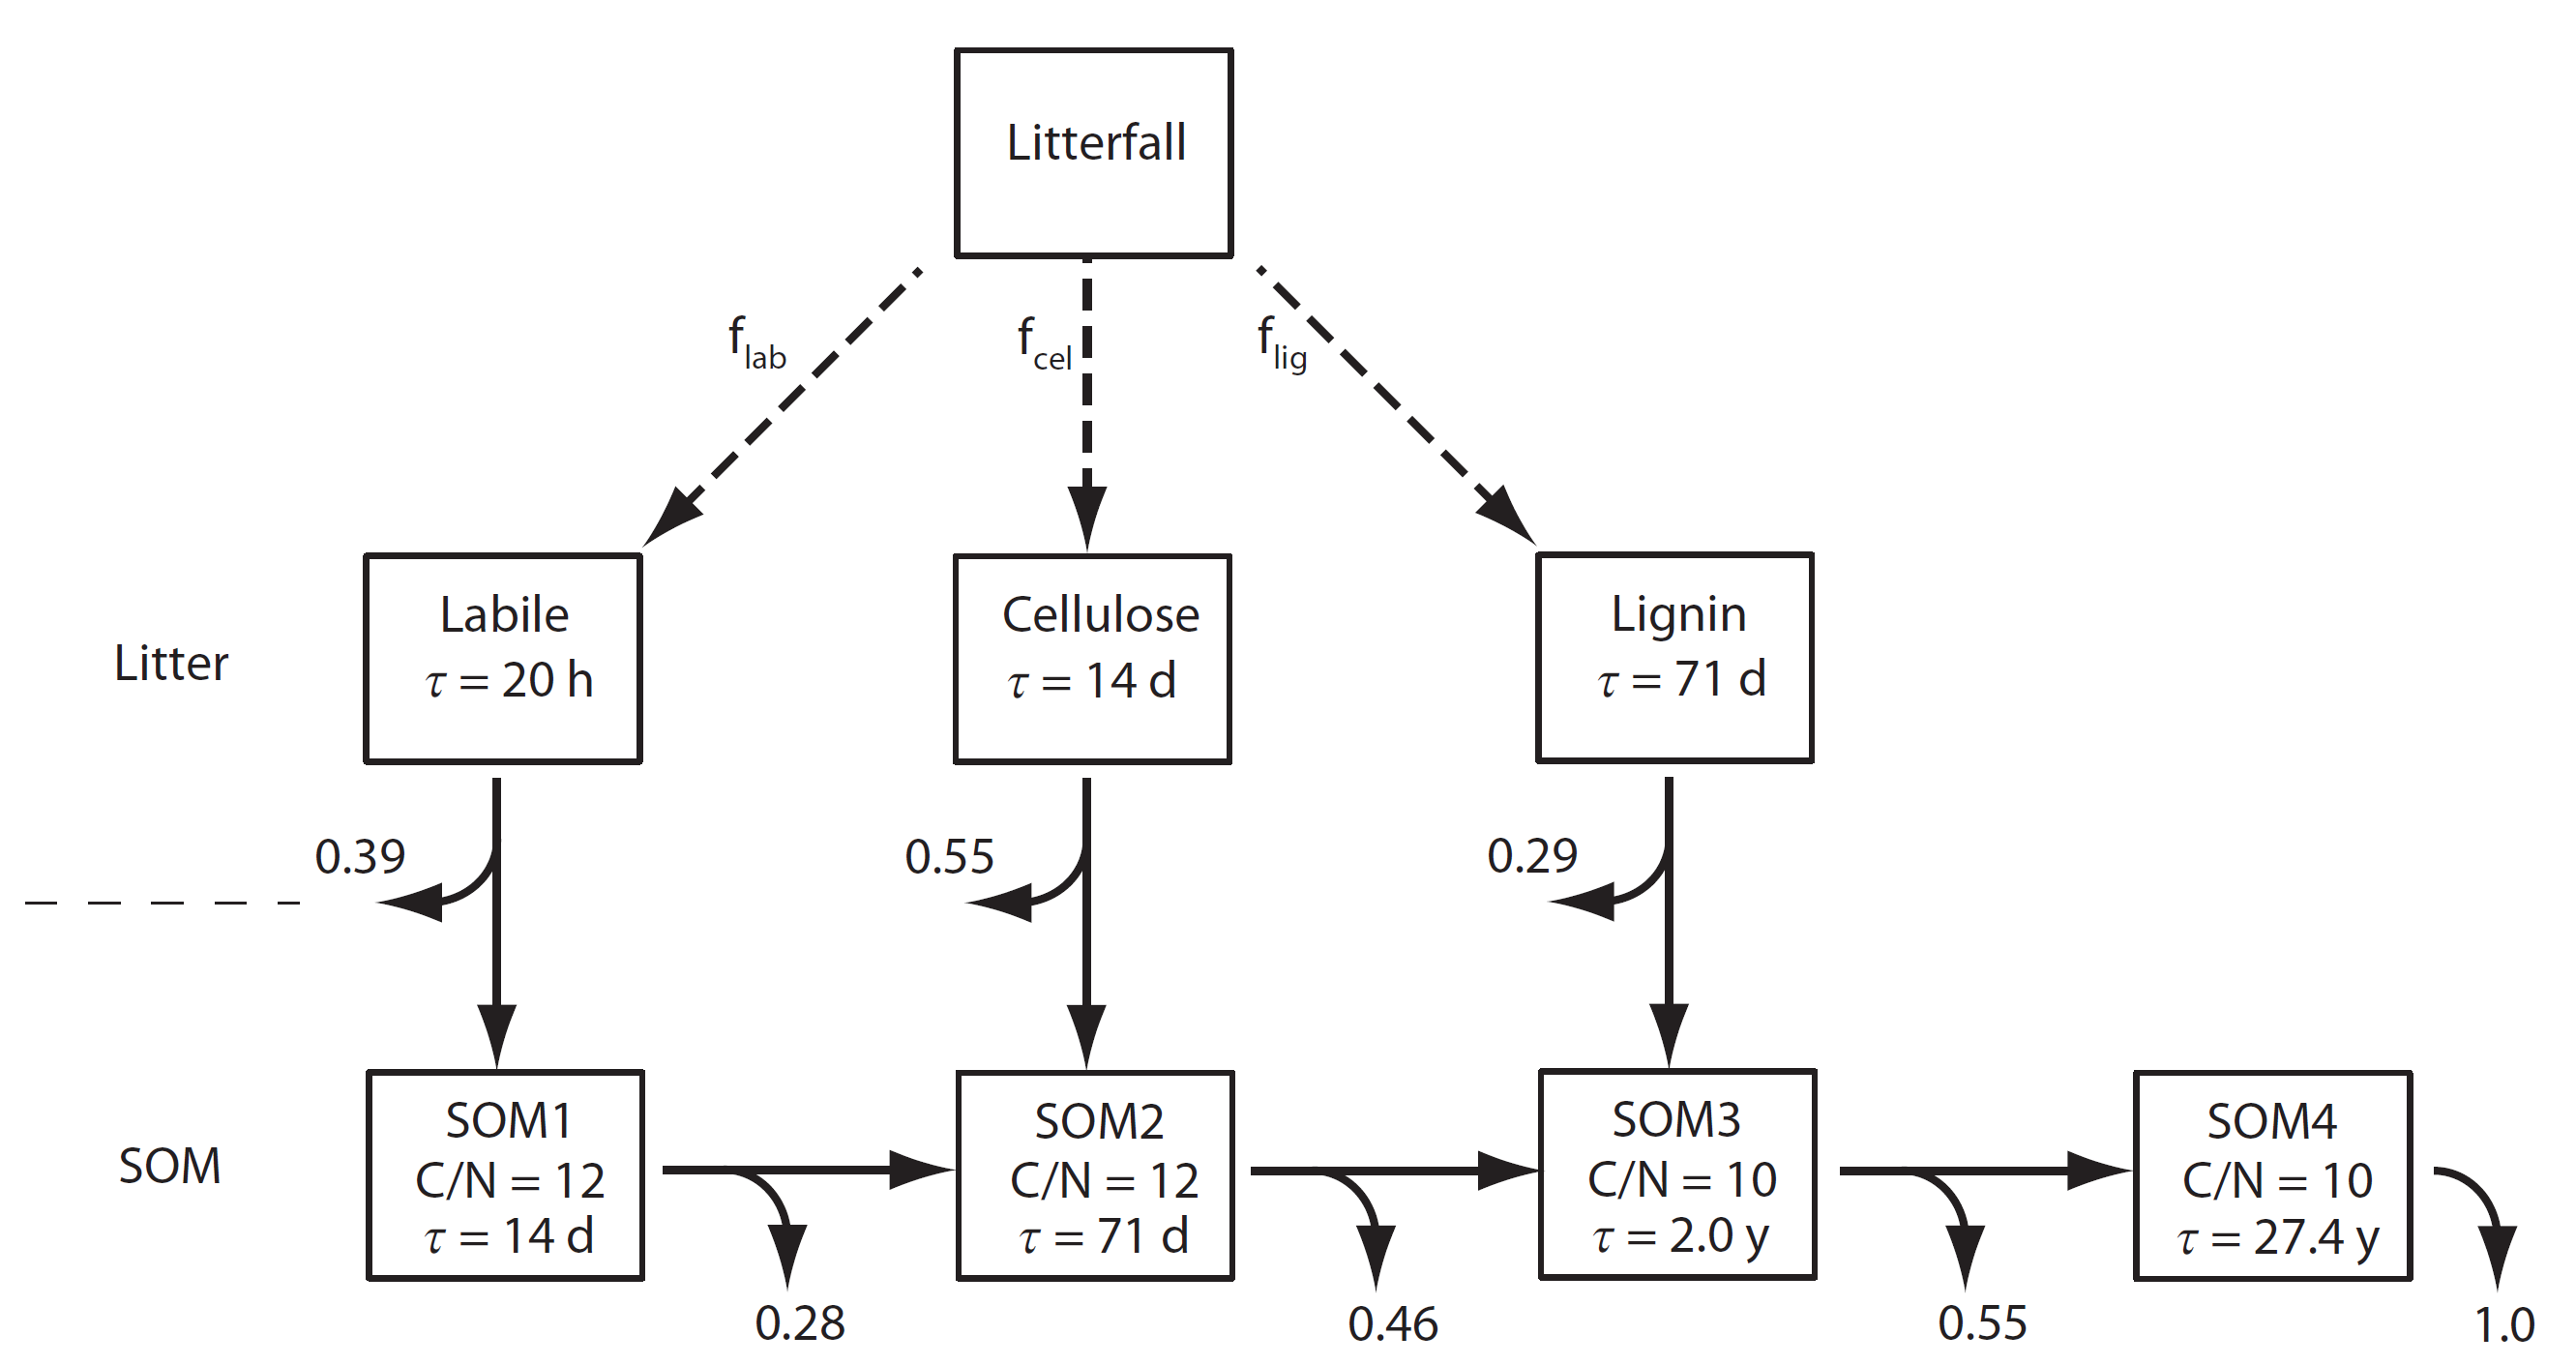
\includegraphics[width=\linewidth]{./CLM-CN_cycle}
}

%-----------------------------------------------------------------------------
\subsection{Governing Equations}

\frame{\frametitle{Reaction Expression}

\Large

\EQ\label{CN_rxn}
\text{CN}_u \eq \left(1-f\right) \text{CN}_d + f \text{CO}_2 + n \text{N}_\text{mineral}
\EN

\EQ\label{n_calc}
n \eq u - \left(1-f\right) d
\EN

\footnotesize
\BA
\text{CN}_u &\eq \text{upstream carbon pool } [\text{mol C}/m^3] \\
\text{CN}_d &\eq \text{downstream carbon pool } [\text{mol C}/m^3] \\
\text{CO}_2 &\eq \text{nitrogen concentration } [\text{mol CO}_2/m^3] \\
\text{N}_\text{mineral} &\eq \text{nitrogen concentration } [\text{mol N}/m^3] \\
u &\eq \text{\text{C}/\text{N} atomic weight ratio divided by upstream \text{C}/\text{N} ratio} \\
d &\eq \text{\text{C}/\text{N} atomic weight ratio divided by downstream \text{C}/\text{N} ratio} \\
f &\eq \text{respiration fraction} \\
\EA
}

\frame{\frametitle{Kinetic Rate Expression}

\Large

\EQ\label{CN_kinetic_rxn}
rate \eq f_T f_\theta f_\text{pi} k \text{CN}_u
\EN

%\bigskip
%\normalsize
%\footnotesize
\scriptsize
\BA
f_T &\eq \exp\left[308.56 \left(\frac{1}{71.02}-\frac{1}{T - 227.13}\right)\right]\\
f_\theta &\eq \frac{\log\left(\theta_\text{min}/\theta\right)}{\log\left(\theta_\text{min}/\theta_\text{max}\right)}\\
f_\text{pi} &\eq \frac{\text{N}_\text{mineral}}{\text{N}_\text{mineral} + K_{\text{N}_\text{mineral}}} \\
k &\eq \text{kinetic rate constant} [s^{-1}]\\
T &\eq \text{temperature } [K] \\
\theta &\eq \text{moisture content or saturation } [-] \\
\text{CN}_u &\eq \text{upstream carbon pool } [\text{mol C}/m^3] \\
\text{N}_\text{mineral} &\eq \text{nitrogen concentration } [\text{mol N}/m^3] \\
K_\text{N} &\eq \text{nitrogen half saturation constant } [\text{mol N}/m^3]\\
\EA

}

\frame{\frametitle{Kinetic Reaction Equations}


\EQ
\text{CN}_u \eq \left(1-f\right) \text{CN}_d + f \text{CO}_2 + n \text{N}_\text{mineral}
\EN

\EQ
rate \eq f_T f_\theta f_\text{pi} k \text{CN}_u
\EN

\Large
\BA
\frac{\p}{\p t} \left(\text{CN}_u\right) &\eq -rate \\
\frac{\p}{\p t} \left(\text{CN}_d\right) &\eq \left(1-f\right) rate \\
\frac{\p}{\p t} \left(\text{CO}_2\right) &\eq f \cdot rate \\
\frac{\p}{\p t} \left(\text{N}_\text{mineral}\right) &\eq n \cdot rate \\
\EA

}


\frame{\frametitle{Newton-Raphson Method}
\LARGE
\BA
\Fb\left(\bx^{k+1,i}\right) &\eq \frac{\bx^{k+1,i}-\bx^k}{\Dt} - \sum_{irxn} \bnu_{irxn} \cdot rate_{irxn} \\
\\
\Jb \dbx &\eq -\Fb\left(\bx^{k+1,i}\right) \\
\\
\bx^{k+1,i+1} &\eq \bx^{k+1,i} + \dbx
\EA
\small
\BA
k &\eq \text{time step} \\
i &\eq \text{iteration}
\EA
}

%-----------------------------------------------------------------------------
\subsection{PFLOTRAN Input Specification}

\begin{frame}[fragile,allowframebreaks]\frametitle{CHEMISTRY}
\small
\begin{semiverbatim}
CHEMISTRY
  ...
  IMMOBILE_SPECIES
    N
    C
    SOM1
    SOM2
    SOM3
    SOM4
    LabileC
    CelluloseC
    LigninC
    LabileN
    CelluloseN
    LigninN
  /
  ...
\end{semiverbatim}
\newpage
\begin{semiverbatim}

  ...
  REACTION_SANDBOX
    CLM-CN
      POOLS   \bluecomment{! CN ratio}
        SOM1   12.d0   \bluecomment{! -> u or d}
        SOM2   12.d0
        SOM3   10.d0
        SOM4   10.d0
        Labile
        Cellulose
        Lignin
      /
      ...
\end{semiverbatim}
\newpage
\begin{semiverbatim}
      ...
      REACTION
        UPSTREAM_POOL Labile         \bluecomment{! CN_u}
        DOWNSTREAM_POOL SOM1         \bluecomment{! CN_d}
        TURNOVER_TIME 20. h          \bluecomment{! -> k}
        RESPIRATION_FRACTION 0.39d0  \bluecomment{! f}
        N_INHIBITION 1.d-10          \bluecomment{! K_N}
      /
      REACTION
        UPSTREAM_POOL SOM1
        DOWNSTREAM_POOL SOM2
        TURNOVER_TIME 14. d
        RESPIRATION_FRACTION 0.28d0
        N_INHIBITION 1.d-10
      /
      ...
    / \bluecomment{! END CLM-CN}
  / \bluecomment{! END REACTION_SANDBOX}
/ \bluecomment{! END CHEMISTRY}
\end{semiverbatim}
\end{frame}

\begin{frame}[fragile]\frametitle{CONSTRAINT}
%\small
\footnotesize
\begin{semiverbatim}
CONSTRAINT initial
  CONCENTRATIONS   \bluecomment{! moles/L}
    A(aq)  1.d-40  T
  /
  IMMOBILE       \bluecomment{! moles/m^3}
    N     1.d-6
    C     1.d-6
    SOM1  1.d-10 \bluecomment{! moles C/m^3}
    SOM2  1.d-10
    SOM3  1.d-10
    SOM4  1.d-10
    LabileC     0.1852d-3
    CelluloseC  0.4578d-3
    LigninC     0.2662d-3
    LabileN     0.00508954d-3
    CelluloseN  0.01258096d-3
    LigninN     0.00731553d-3
  /
END
\end{semiverbatim}
\end{frame}

%-----------------------------------------------------------------------------
\subsection{PFLOTRAN Numerical Implementation}
\frame{\frametitle{Kinetic Reaction Equations}
\BA
\text{Lit1C} + \frac{1}{\text{CN}_{\text{Lit1C}}} {\text {Lit1N}} &\eq \left(1-f_1\right) \text{SOM1} + f_1 \text{CO}_2 + n_1 \text{N}_\text{mineral} \\
\text{Lit2C} + \frac{1}{\text{CN}_{\text{Lit2C}}} {\text {Lit2N}} &\eq \left(1-f_2\right) \text{SOM2} + f_2 \text{CO}_2 + n_2 \text{N}_\text{mineral} \\
\text{Lit3C} + \frac{1}{\text{CN}_{\text{Lit3C}}} {\text {Lit3N}} &\eq \left(1-f_3\right) \text{SOM3} + f_3 \text{CO}_2 + n_3 \text{N}_\text{mineral} \\
\text{SOM1} &\eq \left(1-f_4\right) \text{SOM2} + f_4 \text{CO}_2 + n_4 \text{N}_\text{mineral} \\
\text{SOM2} &\eq \left(1-f_5\right) \text{SOM3} + f_5 \text{CO}_2 + n_5 \text{N}_\text{mineral} \\
\text{SOM3} &\eq \left(1-f_6\right) \text{SOM4} + f_6 \text{CO}_2 + n_6 \text{N}_\text{mineral} \\
\text{SOM4} &\eq f_7 \text{CO}_2 + n_7 \text{N}_\text{mineral} \\
\EA
}

\frame{\frametitle{Kinetic Reaction Equations}

\BA
\text{CN}_{\text{Lit1C}} & \eq  \frac{\text{Lit1C}}{\text{Lit1N}} \\
\text{CN}_{\text{Lit2C}} & \eq \frac{\text{Lit2C}}{\text{Lit2N}} \\
\text{CN}_{\text{Lit3C}} & \eq \frac{\text{Lit3C}}{\text{Lit3N}} \\
\EA

{\begin{center}
\begin{tabular}{ c || c }
  $\text{CN}_{\text{SOM1}} \eq 12$ & $\text{CN}_{\text{SOM2}} \eq 12$  \\
  \hline
  $\text{CN}_{\text{SOM3}} \eq 10$ & $\text{CN}_{\text{SOM4}} \eq 10$  \\
  \hline
  $f_1 \eq 0.39 $ & $f_2 \eq 0.55 $ \\
  \hline
  $f_3 \eq 0.29 $ & $f_4 \eq 0.28 $ \\
  \hline
  $f_5 \eq 0.46 $ & $f_5 \eq 0.55 $ \\
  \hline
  $f_7 \eq 1.0 $ & \\
\end{tabular}
\end{center}
}
}

\frame{\frametitle{Kinetic Reaction Equations}
\BA
n_1 &\eq \frac{1}{\text{CN}_{\text{Lit1C}}} - \left(1-f_1\right) \frac{1}{\text{CN}_{\text{SOM1}}} \\
n_2 &\eq \frac{1}{\text{CN}_{\text{Lit2C}}} - \left(1-f_2\right) \frac{1}{\text{CN}_{\text{SOM2}}} \\
n_3 &\eq \frac{1}{\text{CN}_{\text{Lit3C}}} - \left(1-f_3\right) \frac{1}{\text{CN}_{\text{SOM3}}} \\
n_4 &\eq \frac{1}{\text{CN}_{\text{SOM1}}} - \left(1-f_4\right) \frac{1}{\text{CN}_{\text{SOM2}}} \\
n_5 &\eq \frac{1}{\text{CN}_{\text{SOM2}}} - \left(1-f_5\right) \frac{1}{\text{CN}_{\text{SOM3}}} \\
n_6 &\eq \frac{1}{\text{CN}_{\text{SOM3}}} - \left(1-f_6\right) \frac{1}{\text{CN}_{\text{SOM4}}} \\
n_7 &\eq \frac{1}{\text{CN}_{\text{SOM4}}} 
\EA
}

\frame{\frametitle{Kinetic Reaction Equations}
\BA
R_1 \eq f_T f_\theta f_\text{pi} k \text{Lit1C} \\
R_2 \eq f_T f_\theta f_\text{pi} k \text{Lit2C} \\
R_3 \eq f_T f_\theta f_\text{pi} k \text{Lit3C} \\
R_4 \eq f_T f_\theta f_\text{pi} k \text{SOM1} \\
R_5 \eq f_T f_\theta f_\text{pi} k \text{SOM2} \\
R_6 \eq f_T f_\theta f_\text{pi} k \text{SOM3} \\
R_7 \eq f_T f_\theta f_\text{pi} k \text{SOM4} 
\EA
}


\frame{\frametitle{Mass Conservation Equations}
The CLM-CN reaction network results in 12 basis species for which the mass conservation equation are given by: 
\BA
\frac{\p}{\p t} \left(\text{N}_\text{mineral}\right) &\eq n_1R_1 + n_2R_2 + n_3R_3 +n_4R_4 +n_5R_5 +n_6R_6 + n_7R_7 \\
\frac{\p}{\p t} \left(\text{CO}_2\right) &\eq  f_1R_1 + f_2R_2 + f_3R_3 + f_4R_4 + f_5R_5 + f_6R_6 + f_7R_7 \\
\frac{\p}{\p t} \left(\text{SOM1}\right) &\eq  (1-f_1)R_1 - R_4\\
\frac{\p}{\p t} \left(\text{SOM2}\right) &\eq  (1-f_2)R_2 + (1-f_4)R_4 - R_5\\
\frac{\p}{\p t} \left(\text{SOM3}\right) &\eq  (1-f_3)R_3 + (1-f_5)R_5 - R_6\\
\frac{\p}{\p t} \left(\text{SOM4}\right) &\eq  (1-f_6)R_6 - R_7
\EA
}

\frame{\frametitle{Mass Conservation Equations}
\BA
\frac{\p}{\p t} \left(\text{Lit1C}\right) &\eq  -R_1 \\
\frac{\p}{\p t} \left(\text{Lit2C}\right) &\eq  -R_2 \\
\frac{\p}{\p t} \left(\text{Lit3C}\right) &\eq  -R_3 \\
\frac{\p}{\p t} \left(\text{Lit1N}\right) &\eq   \frac{-1}{\text{CN}_{\text{Lit1C}}}R_1\\
\frac{\p}{\p t} \left(\text{Lit3N}\right) &\eq  \frac{-1}{\text{CN}_{\text{Lit2C}}}R_2 \\
\frac{\p}{\p t} \left(\text{Lit3N}\right) &\eq  \frac{-1}{\text{CN}_{\text{Lit3C}}}R_3 
\EA
}

\frame{\frametitle{Numerical Implementation in PFLOTRAN}
Applying finite-volume spatial discretization on mass conservation equation for Lit1C:
\EQ
\int \frac{\p}{\p t} \left(\text{Lit1C}\right) dV \eq  \int -R_1 dV
\EN

\EQ
\frac{\p}{\p t} \left(\text{Lit1C }\Delta V\right)  \eq   -R_1 \Delta V
\EN

Implicit time discretization:
\EQ
\frac{\Delta V}{\Delta t} \left(\text{Lit1C}^{t+1} - \text{Lit1C}^t\right)  \eq   -R_1^{t+1} \Delta V
\EN

Residual equation:
\EQ
\mathcal{R}_7 \eq  \frac{\Delta V}{\Delta t} \left(\text{Lit1C}^{t+1} - \text{Lit1C}^t\right)  + R_1^{t+1} \Delta V
\EN
Note: The residual equation for Lit1C is $\mathcal{R}_7$ since Lit1C is the 7-th basis specie
}

\frame{\frametitle{Numerical Implementation in PFLOTRAN}
Jacobian for Lit1C:
\BA
\mathcal{J}_{7,7} & \eq \frac{\p \mathcal{R}_7 }{\p \left(\text{Lit1C}^{t+1} \right)} \\
\mathcal{J}_{7,1} & \eq \frac{\p \mathcal{R}_7 }{\p \left(\text{N}_\text{mineral}^{t+1} \right)} \\
\mathcal{J}_{7,i} & \eq 0 \text{\hspace{2cm}i $\neq 1, 7$ }
\EA
}

\end{document}
